\chapter{कशेरुकियों का भ्रूणीय विकास}\label{ch:b2:vertebrate-development}

मेंढक का अंडाणु दो मिलिमीटर चौड़ा एक गोला है, ऊपर से गहरा और
नीचे से फीका। दिन भर में वह हज़ारों कोशिकाओं में बँट जाता है; दो दिन में
उन्हीं कोशिकाओं की एक चादर किसी खाँचे से होकर भीतर लुढ़ककर एक आँत बना
लेती है और पीठ के साथ एक छड़ बिछा देती है; और तीन दिन में उस छड़ के ऊपर
की चादर मुड़कर ऐसी नली बन जाती है जो मस्तिष्क और मेरुरज्जु बनेगी। जल के
सिवा कुछ भी नहीं जोड़ा गया। जो सूचना एक कोशिका को तैरते भेक-शिशु में बदल
देती है वह उस अंडाणु में और उसके जीनोम में थी, और जिस ढंग से वह खुलती है
--- \omterm{def:b2:vertebrate-development:egg}{विदलन}, गैस्ट्रुलन, तंत्रिकायन, और पड़ोसियों द्वारा हर भाग का \omterm{def:b2:vertebrate-development:induction}{प्रेरण}
--- वह किसी मछली, किसी चूज़े और किसी चूहे में पहचान लेने लायक़ एक ही है।
यह अध्याय किसी कशेरुकी भ्रूण का इन चरणों के आरपार पीछा करता है और उन
प्रयोगों का वर्णन करता है जिन्होंने दिखाया कि उसके हर भाग को क्या बनना है यह कैसे बताया जाता है।

\section{अंडाणु से कोरकपुटी तक}

\begin{definition}[अंडाणु और उसकी अक्षें]\label{def:b2:vertebrate-development:egg}
\index{प्राणी ध्रुव}\index{वनस्पति ध्रुव}\index{पीतक}\index{विदलन}
कशेरुकी अंडाणु निषेचन से पहले ही ध्रुवित है:
\emph{प्राणी ध्रुव} केंद्रक और अधिकांश कोशिकाद्रव्य रखता है, और
\emph{वनस्पति ध्रुव} \emph{पीतक}, यानी प्रोटीन तथा लिपिड का वह भंडार
जिस पर वह भ्रूण खाने लगने तक जीएगा। पीतक की मात्रा
आगे की हर बात का ढाँचा तय कर देती है: समुद्री अर्चिन या स्तनधारी के
अंडाणु में लगभग कुछ नहीं होता और वह पूरा का पूरा बराबर कोशिकाओं में
विदलित होता है; मेंढक के अंडाणु में मध्यम मात्रा होती है और वह पूरा तो
विदलित होता है पर असमान रूप से (ऊपर छोटी कोशिकाएँ, नीचे बड़ी पीतकी
कोशिकाएँ); और मछली या पक्षी का अंडाणु लगभग पूरा पीतक है और केवल उसके
ऊपर कोशिकाद्रव्य की एक चक्रिका में विदलित होता है।
मेंढक में जहाँ शुक्राणु घुसता है वही बिंदु दूसरी अक्ष तय कर देता है:
बाह्यक उससे तीस अंश घूम जाता है और प्रवेश-बिंदु के सामने एक
\emph{धूसर अर्धचंद्र} उघाड़ देता है, और वही ओर पीठ
बनेगी। \emph{विदलन} बिना किसी वृद्धि के तेज़ समसूत्री विभाजनों की एक
शृंखला है --- हर बार कोशिकाएँ आधी हो जाती हैं --- जो अंडाणु में सँजोए
मातृ mRNA तथा प्रोटीनों से चलती है, और भ्रूण के अपने जीन
\emph{मध्य-कोरकपुटी संक्रमण} तक चुप रहते हैं, यानी कोई बारह
विभाजन तक।
\end{definition}

\begin{omfigure}
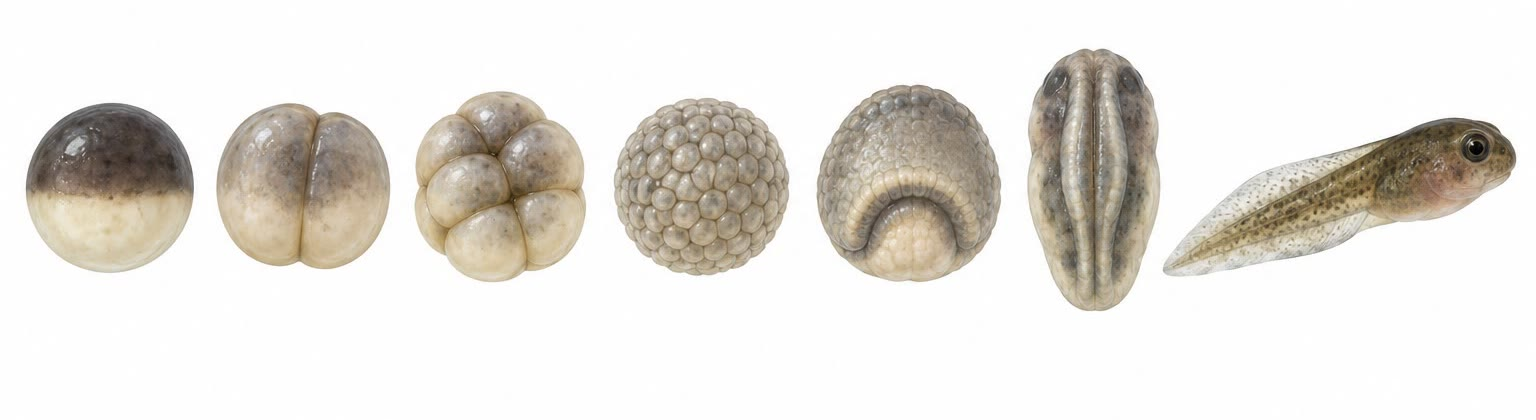
\includegraphics[width=0.9\linewidth]{images/book4/ai/b4-10-frog-development.jpg}

{\small किसी निषेचित अंडाणु से मेंढक का विकास: \omterm{def:b2:vertebrate-development:egg}{विदलन} से
\omterm{def:b2:vertebrate-development:blastula}{कोरकपुटी} तक, गैस्ट्रुलन, तंत्रिका वलनों सहित न्यूरुला, और
भेक-शिशु --- सब कुछ कुछ ही दिनों में, बिना किसी वृद्धि के।}
\end{omfigure}

\begin{theorem}[विदलन का अंकगणित]\label{thm:b2:vertebrate-development:cleavage}
$k$ समकालिक \omterm{def:b2:vertebrate-development:egg}{विदलनों} के बाद $V_0$ आयतन का अंडाणु $2^{k}$
कोशिकाएँ बन जाता है, जिनका माध्य आयतन $V_0/2^{k}$ और त्रिज्या
$r_0/2^{k/3}$ है, और कुल पृष्ठ $2^{k/3}$ गुना बढ़ जाता है; और
केंद्रकीय से कोशिकाद्रव्यी आयतन का अनुपात, जो मेंढक के अंडाणु में
$10^{-4}$ के पास से आरंभ होता है, $2^{k}$ गुना चढ़ता है और लगभग दस
विभाजनों के बाद किसी साधारण कोशिका के अनुपात ($\sim 0.1$) तक पहुँच जाता
है। यही चढ़ता अनुपात --- यानी किसी नियत मातृ भंडार के किसी संदमक का
चरघातांकी रूप से बढ़ती DNA मात्रा से अनुमापन --- मध्य-कोरकपुटी संक्रमण
का चालक है: विभाजन धीमे और असमकालिक हो जाते हैं, और युग्मनजी जीनोम
चालू हो जाता है।
\end{theorem}
\begin{proof}
\omterm{def:b2:vertebrate-development:egg}{विदलन} में आयतन संरक्षित रहता है, इसलिए $2^{k}$ कोशिकाओं में से हर एक का $V_0
2^{-k}$ है और, गोला मानकर, त्रिज्या $r_0 2^{-k/3}$; और उनका कुल
क्षेत्रफल $2^{k}\cdot 4\pi r_0^{2}\, 2^{-2k/3} = 4\pi r_0^{2}\, 2^{k/3}$ है। हर
कोशिका नियत आकार का एक केंद्रक रखती है, इसलिए वह अनुपात
$2^{k}$ की तरह बढ़ता है, $10^{-4}$ से: $2^{10} = 1024$ उसे $0.1$ तक ले आता है। मेंढक का
संक्रमण बारहवें विभाजन पर पड़ता है, जो थोड़ी देर से पहुँचती किसी
देहली के अनुरूप है।
\end{proof}
\begin{proof}[प्रमाण-सामग्री]
न्यूपोर्ट और किर्शनर (1982) ने मेंढक के अंडाणुओं में अतिरिक्त DNA डाला
और पाया कि वह संक्रमण उतने ही विभाजन पहले आ गया जितना DNA अधिक था; और
कोशिकाद्रव्य हटाने का भी वही प्रभाव हुआ। वह घड़ी न काल है, न विभाजनों की
गिनती, बल्कि एक अनुपात है।
\end{proof}

\begin{definition}[कोरकपुटी]\label{def:b2:vertebrate-development:blastula}
\index{कोरकपुटी (उभयचर)}\index{कोरकगुहा}
\omterm{def:b2:vertebrate-development:egg}{विदलन} का अंत \emph{कोरकपुटी} पर होता है: यानी किसी गुहा के, यानी
\emph{कोरकगुहा} के, चारों ओर कुछ हज़ार कोशिकाओं की एक खोखली गेंद (मेंढक,
समुद्री अर्चिन) या एक चक्रिका (मछली, पक्षी)। उसकी कोशिकाएँ देखने में अब
भी अविशिष्ट हैं, पर वे समतुल्य नहीं हैं: सतह के टुकड़ों को रंजकों से
रँगकर और उनका पीछा करके बनाया गया कोई \emph{नियति-मानचित्र} दिखाता है कि
प्राणी टोपी त्वचा और तंत्रिका तंत्र देगी (\emph{बाह्यचर्म}), विषुवती
पट्टी पेशी, कंकाल, वृक्क तथा रक्त
(\emph{मध्यचर्म}), और वनस्पति पिंड आँत तथा उसके अंग
(\emph{अंतश्चर्म})। ये तीनों \emph{जनन स्तर} हर
कशेरुकी में एक ही हैं, और अगला पग उन्हें उनकी जगह पर बिठाना है:
मध्यचर्म और अंतश्चर्म बाहर हैं और उन्हें भीतर जाना है।
\end{definition}

\section{गैस्ट्रुलन और तंत्रिकायन}

\begin{proposition}[गैस्ट्रुलन]\label{prop:b2:vertebrate-development:gastrulation}
\index{गैस्ट्रुलन}\index{कोरकरंध्र}\index{आद्यांत्र}\index{पृष्ठरज्जु}
\emph{गैस्ट्रुलन} कोशिका-गतियों का वह समुच्चय है जो एक-परती
\omterm{def:b2:vertebrate-development:blastula}{कोरकपुटी} को तीन-परती \emph{गैस्ट्रुला} में बदल देता है। मेंढक में
वह धूसर अर्धचंद्र के नीचे आरंभ होता है: वहाँ की कोशिकाएँ अपना आकार बदलती
हैं, अपने बाहरी सिरे सिकोड़कर बोतल जैसी हो जाती हैं, और वह सतह एक
खाँचे में, यानी \emph{कोरकरंध्र} में, धँस जाती है। उसी से मध्यचर्म और
अंतश्चर्म भीतर बहते हैं (\emph{अंतर्वलन}), उस ओष्ठ पर लुढ़कते हुए
और गुहा की छत के साथ आगे बढ़ते हुए; प्राणी टोपी नीचे फैलकर बाहर ढक
लेती है (\emph{अधिवर्धन}); और वह कोरकरंध्र सिकुड़कर अंतिम पीतकी कोशिकाओं
के चारों ओर एक वलय रह जाता है। भीतर, अंतश्चर्म से अस्तरित एक नई गुहा,
यानी \emph{आद्यांत्र}, भावी आँत है, और जो मध्यचर्म सबसे पहले भीतर
लुढ़का, मध्यरेखा के साथ, वह एक कड़ी छड़, यानी \emph{पृष्ठरज्जु}, बन चुका
है, जो हर कशेरुकी भ्रूण की अक्ष है और वही संरचना जिस पर उस संघ का नाम
है। पक्षियों और स्तनधारियों में वही गतियाँ किसी चपटी चक्रिका में एक
दरार, यानी \emph{आद्य रेखा}, से होकर होती हैं; और मछली में वह चक्रिका
\omterm{def:b2:vertebrate-development:egg}{पीतक} के ऊपर फैल जाती है। नृत्य-विन्यास \omterm{def:b2:vertebrate-development:egg}{पीतक} के साथ बदलता है; पर परिणाम
--- बाहर बाह्यचर्म, आँत को अस्तरित करता अंतश्चर्म, बीच में मध्यचर्म,
मध्यरेखा में पृष्ठरज्जु --- वही रहता है।
\end{proposition}

\begin{omfigure}
\begin{tikzpicture}[every node/.style={font=\scriptsize}, >=stealth]
  % blastula
  \begin{scope}
    \draw[thick, fill=omDef!15] (0,0) circle (1.3);
    \draw[thick, fill=white] (0,0.2) circle (0.75);
    \fill[omExo!40] (0,0) ++(-1.3,0) arc (180:360:1.3 and 1.3) -- cycle;
    \draw[thick] (0,0) circle (1.3);
    \node at (0,0.2) {कोरकगुहा};
    \node[below, align=center] at (0,-1.45) {कोरकपुटी\\प्राणी टोपी (नीली), पीतकी कोशिकाएँ (धूसर)};
  \end{scope}
  % early gastrula: blastopore forming
  \begin{scope}[xshift=4.2cm]
    \draw[thick, fill=omDef!15] (0,0) circle (1.3);
    \draw[thick, fill=white] (0,0.25) circle (0.7);
    \fill[omExo!40] (0,0) ++(-1.3,0) arc (180:360:1.3 and 1.3) -- cycle;
    \draw[thick] (0,0) circle (1.3);
    \draw[very thick, omThm] (1.0,-0.85) .. controls (0.5,-0.6) and (0.4,-0.3) .. (0.55,0.0);
    \draw[->, thick, omThm] (1.15,-0.7) .. controls (0.6,-0.4) .. (0.4,0.1);
    \draw[omThm] (1.0,-0.85) -- (0.9,-1.25); \node[omThm, anchor=north west] at (0.6,-1.2) {कोरकरंध्र-ओष्ठ};
    \node[below, align=center] at (0,-1.45) {आरंभिक गैस्ट्रुला\\कोशिकाएँ ओष्ठ पर लुढ़ककर भीतर जाती हैं};
  \end{scope}
  % late gastrula
  \begin{scope}[xshift=8.4cm]
    \draw[thick, fill=omDef!15] (0,0) circle (1.3);
    \draw[thick, fill=omExo!25] (0,0.05) circle (0.95);
    \draw[thick, fill=white] (0.15,-0.1) ellipse (0.55 and 0.4);
    \draw (0.6,-0.3) -- (1.6,-1.15); \node[anchor=west] at (1.6,-1.15) {आद्यांत्र};
    \draw[very thick, omThm] (-0.9,0.35) .. controls (-0.2,0.6) .. (0.8,0.4);
    \draw[omThm] (0.0,0.48) -- (-0.9,1.55); \node[omThm, anchor=east] at (-0.9,1.55) {पृष्ठरज्जु};
    \draw[thick] (1.1,-0.7) -- (1.3,-0.5);
    \node[right] at (1.3,-0.5) {कोरकरंध्र};
    \node[below, align=center] at (0,-1.45) {पश्च गैस्ट्रुला: तीन परतें,\\आँत-गुहा, छत पर पृष्ठरज्जु};
  \end{scope}
\end{tikzpicture}

{\small मेंढक में गैस्ट्रुलन, काट में। कोशिकाएँ कोरकरंध्र के ओष्ठ पर
भीतर लुढ़कती हैं; अंतश्चर्म एक नई आँत-गुहा को अस्तरित करता है, और जो
मध्यचर्म पहले घुसता है वह मध्यरेखा के साथ पृष्ठरज्जु बन जाता है।}
\end{omfigure}

\begin{proposition}[तंत्रिकायन और शरीर-योजना]\label{prop:b2:vertebrate-development:neurulation}
\index{तंत्रिकायन}\index{तंत्रिका नली}\index{कायखंड}\index{तंत्रिका शिखा}
पृष्ठरज्जु के ऊपर का बाह्यचर्म मोटा होकर एक \emph{तंत्रिका
पट्ट} बन जाता है, जिसके किनारे वलनों की तरह उठते हैं और मध्यरेखा में
मिलकर \emph{\omterm{prop:b2:vertebrate-development:neurulation}{तंत्रिका नली}} बनाते हैं, यानी भावी मस्तिष्क तथा मेरुरज्जु,
जो त्वचा के नीचे धँस जाती है; और उन वलनों की चोटी की कोशिकाएँ, यानी
\emph{\omterm{prop:b2:vertebrate-development:neurulation}{तंत्रिका शिखा}}, दूर जाकर परिधीय तंत्रिकाएँ,
वर्णक कोशिकाएँ, अधिवृक्क मज्जा और चेहरे का अधिकांश भाग बनाती हैं।
पृष्ठरज्जु के दोनों ओर मध्यचर्म खंडों में, यानी
\emph{कायखंडों} में, बँट जाता है, जो सिर से पूँछ तक एक के बाद एक जोड़े
में बनते हैं और कशेरुक, धड़ की पेशियाँ तथा चर्म देते हैं; पार्श्व
मध्यचर्म उन परतों में बँट जाता है जो देहगुहा को अस्तरित करती हैं और
हृदय तथा अंग बनाती हैं; और अंतश्चर्म की नली से फेफड़े, यकृत तथा
अग्न्याशय मुकुलित होते हैं। तंत्रिकायन के अंत तक उस भ्रूण के पास
कशेरुकी शरीर-योजना है --- किसी पृष्ठरज्जु के ऊपर एक पृष्ठीय तंत्रिका
रज्जु, एक अधर आँत, खंडित पेशी, एक सिर --- और वह भी कुछ मिलिमीटर की
लंबाई पर, और बाक़ी विकास इसी योजना से अंगों का विस्तार है
(\cref{ch:b2:limb-organogenesis})।
\end{proposition}

\begin{omfigure}
\begin{tikzpicture}[every node/.style={font=\scriptsize}]
  \foreach \x/\lab in {0/{तंत्रिका पट्ट}, 4.0/{तंत्रिका वलन उठते हैं}, 8.0/{तंत्रिका नली बंद; तंत्रिका शिखा प्रवास करती है}} {
    \begin{scope}[xshift=\x cm]
      \draw[thick, fill=omExo!25] (-1.6,0) rectangle (1.6,-1.6);
      \draw[thick, omThm, fill=omThm!30] (0,-0.75) circle (0.28);
      \draw[thick, fill=omProp!30] (-1.3,-0.75) circle (0.32); \draw[thick, fill=omProp!30] (1.3,-0.75) circle (0.32);
      \node[below, align=center, text width=3.4cm] at (0,-1.7) {\lab};
    \end{scope}
  }
  \draw[very thick, omDef] (-1.6,0) -- (-0.7,0) .. controls (-0.3,0.15) and (0.3,0.15) .. (0.7,0) -- (1.6,0);
  \draw[very thick, omDef] (2.4,0) -- (3.3,0) .. controls (3.3,0.9) and (3.6,0.1) .. (4.0,0.0) .. controls (4.4,0.1) and (4.7,0.9) .. (4.7,0) -- (5.6,0);
  \draw[very thick, omDef] (6.4,0.05) -- (9.6,0.05);
  \draw[very thick, omDef, fill=omDef!20] (8.0,-0.3) circle (0.3);
  \foreach \p in {(7.35,-0.4),(8.65,-0.4)} \fill[omDef!70!black] \p circle (0.07);
  \node[omThm, anchor=west] at (9.8,-0.75) {पृष्ठरज्जु};
  \node[omProp, anchor=west] at (9.8,-1.15) {कायखंड};
  \node[omDef, anchor=west] at (9.8,-0.3) {तंत्रिका नली};
  \node[omDef!70!black, anchor=west] at (9.8,0.1) {तंत्रिका शिखा कोशिकाएँ};
\end{tikzpicture}

{\small अनुप्रस्थ काट में तंत्रिकायन: पृष्ठरज्जु (लाल) के ऊपर का
बाह्यचर्म मोटा होता है, मुड़ता है और \omterm{prop:b2:vertebrate-development:neurulation}{तंत्रिका नली}
(नीली) में बंद हो जाता है, जबकि पृष्ठरज्जु के बग़ल का मध्यचर्म
कायखंडों (नारंगी) में बँटता है और \omterm{prop:b2:vertebrate-development:neurulation}{तंत्रिका शिखा} की कोशिकाएँ बंद होते वलनों से निकल जाती हैं।}
\end{omfigure}

\begin{omfigure}
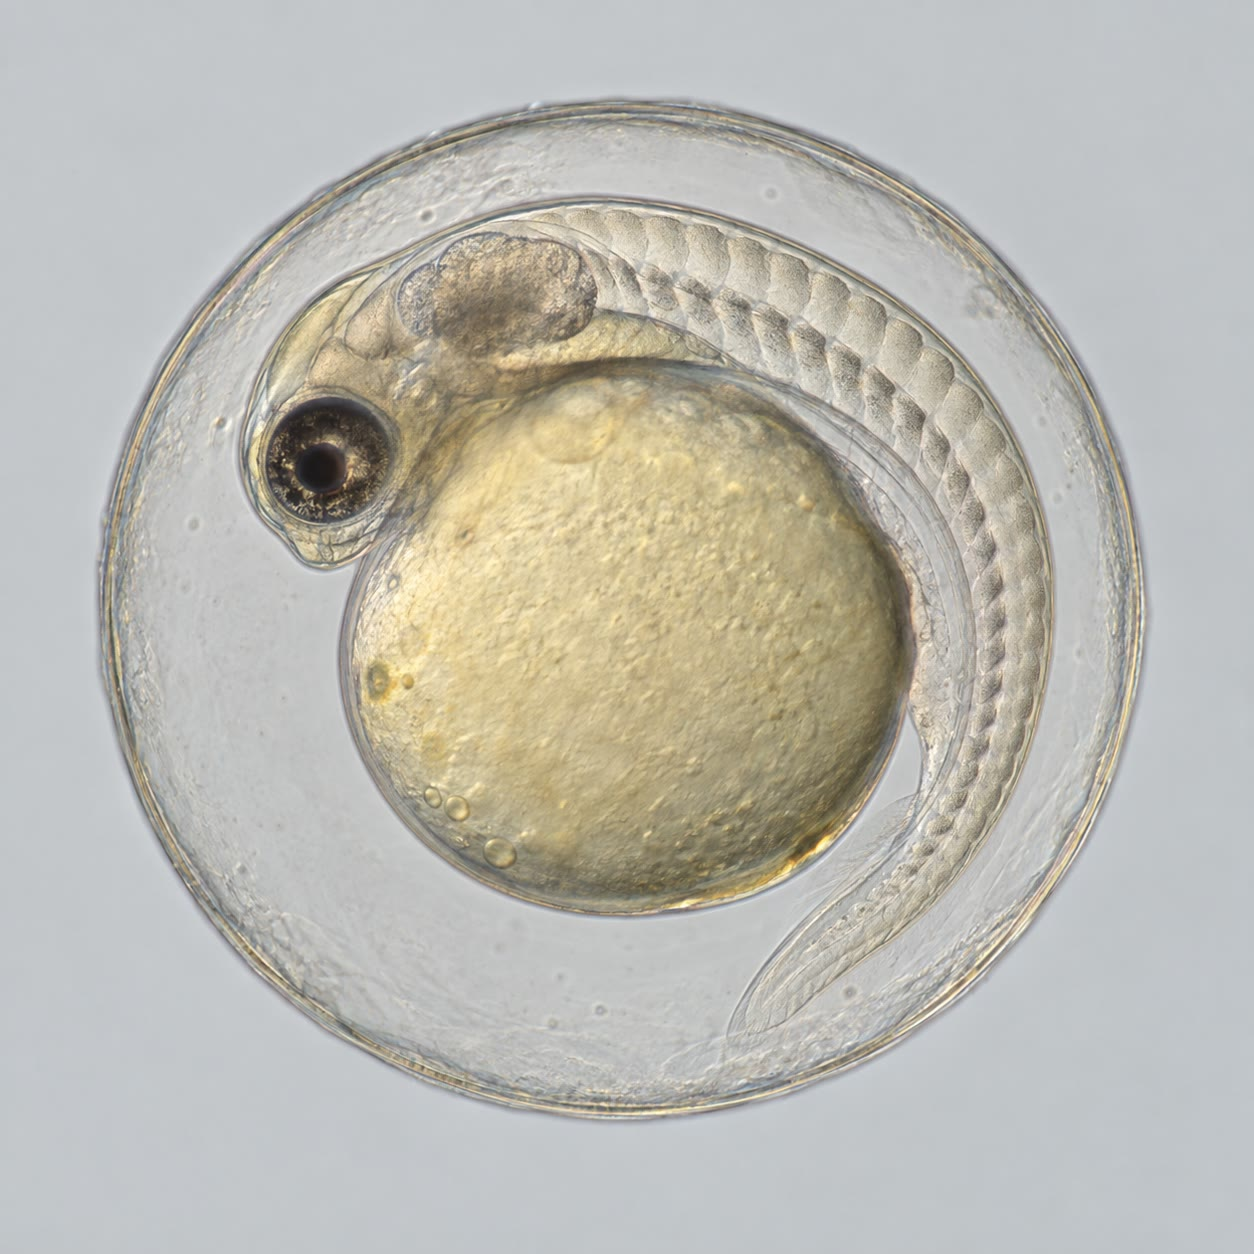
\includegraphics[width=0.42\linewidth]{images/book4/ai/b4-10-zebrafish-embryo.jpg}\hspace{0.04\linewidth}
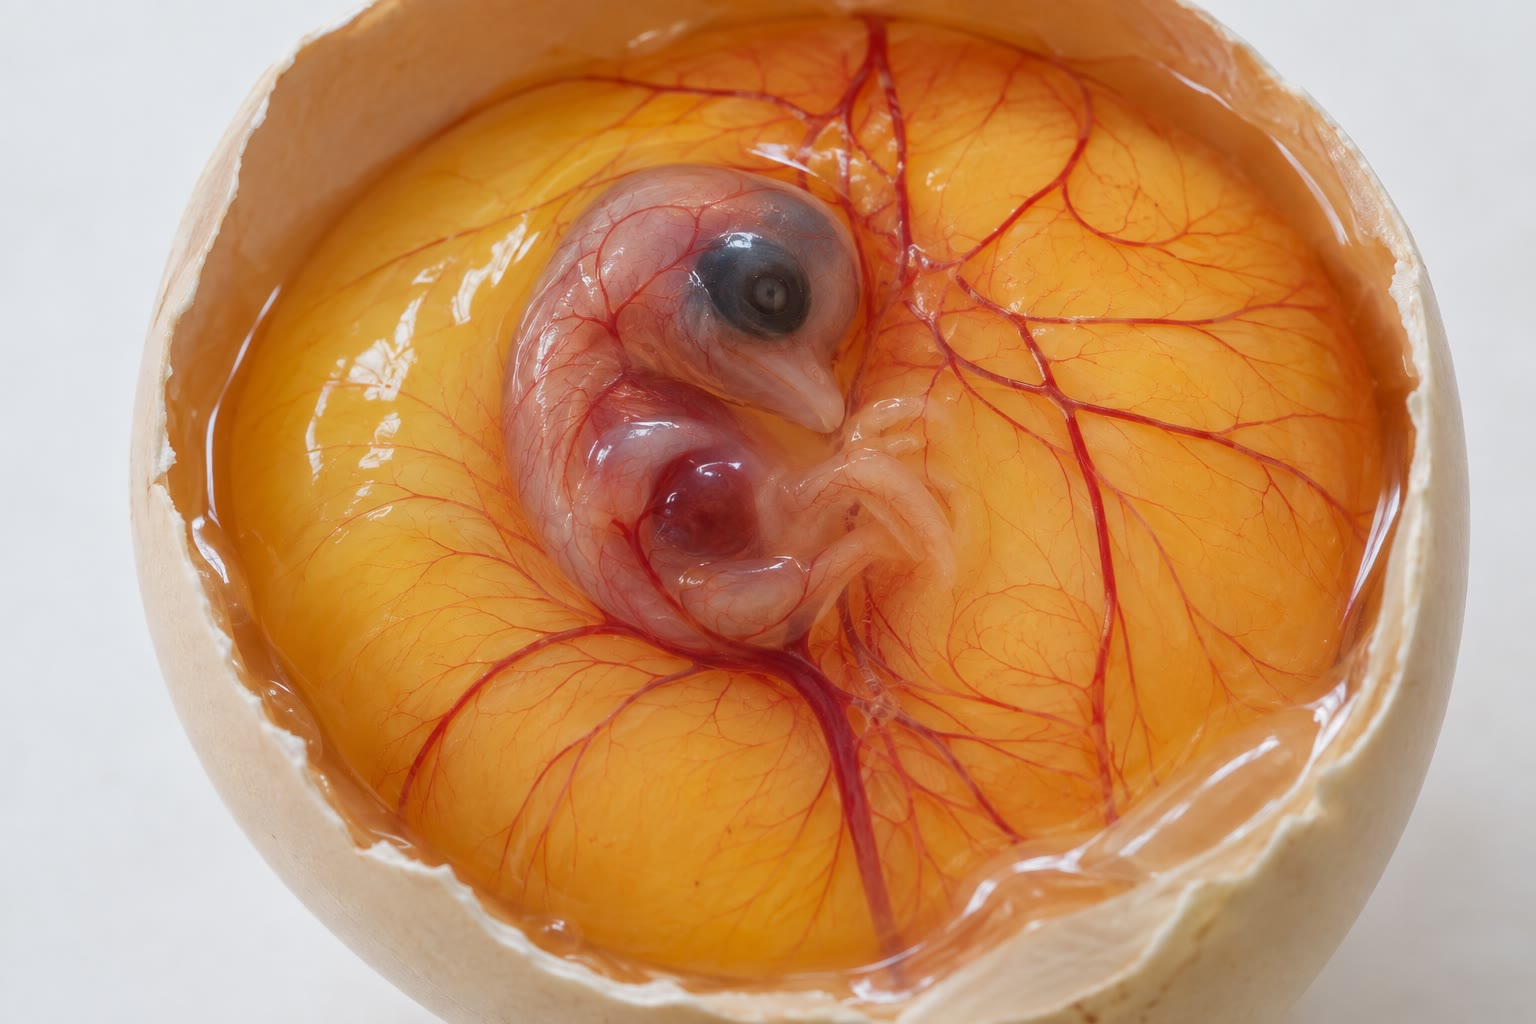
\includegraphics[width=0.5\linewidth]{images/book4/ai/b4-10-chick-embryo.jpg}

{\small बाएँ: अपने जरायु के भीतर एक दिन का कोई ज़ेब्राफ़िश भ्रूण,
अपने \omterm{def:b2:vertebrate-development:egg}{पीतक} के चारों ओर सिमटा, आँख, मस्तिष्क और कायखंडों की एक पंक्ति
सहित। दाएँ: अपने \omterm{def:b2:vertebrate-development:egg}{पीतक} पर तीन दिन का कोई चूज़ा-भ्रूण, जिसका हृदय पहले ही
धड़क रहा है और जिसकी वाहिकाएँ उसे खिलाने को \omterm{def:b2:vertebrate-development:egg}{पीतक} पर फैल रही हैं।}
\end{omfigure}

\section{प्रेरण: कोशिकाएँ कैसे जानती हैं कि वे कहाँ हैं}

\begin{definition}[प्रेरण और सक्षमता]\label{def:b2:vertebrate-development:induction}
\index{प्रेरण (भ्रूणीय)}\index{सक्षमता}\index{संघटक}
\emph{प्रेरण} वह प्रक्रिया है जिससे कोशिकाओं का एक समूह किसी संकेत से
किसी पड़ोसी समूह की नियति बदल देता है; और उत्तर देती कोशिकाओं को
\emph{सक्षम} होना चाहिए --- यानी उत्तर दे पाना, जो वे केवल सीमित काल तक
ही होती हैं। विकास प्रेरणों की एक शृंखला है: वनस्पति
कोशिकाएँ अपने ऊपर की कोशिकाओं में मध्यचर्म प्रेरित करती हैं; पृष्ठीय
मध्यचर्म --- यानी कोरकरंध्र-ओष्ठ का \emph{संघटक} --- अपने ऊपर के
बाह्यचर्म में तंत्रिका पट्ट प्रेरित करता है और दोनों ओर के मध्यचर्म को
ढाँचा देता है; पृष्ठरज्जु \omterm{prop:b2:vertebrate-development:neurulation}{तंत्रिका नली} का तल प्रेरित करता है;
नेत्र पुटिका, जो मस्तिष्क की एक कली है, जिस त्वचा को छूती है उसमें
लेंस प्रेरित करती है; और वह लेंस स्वच्छपटल प्रेरित करता है। हर प्रेरित
ऊतक अगले का प्रेरक बन जाता है। संकेत स्रावी प्रोटीनों के मुट्ठी भर कुल
हैं, जो बार-बार काम में आते हैं --- और वही जो किसी अंग को ढाँचा देते हैं
(\cref{ch:b2:limb-organogenesis}) और, वयस्क में,
\cref{ch:b2:cell-signalling} का संकेतन चलाते हैं।
\end{definition}
\begin{proof}[प्रमाण-सामग्री]
स्पेमान और मांगोल्ड (1924) ने किसी न्यूट जाति के आरंभिक गैस्ट्रुला से
पृष्ठीय कोरकरंध्र-ओष्ठ काटकर किसी दूसरी जाति के अधर
भाग पर ग्राफ़्ट किया, और वह दूसरी जाति भिन्न रंजित थी ताकि पोषी तथा
ग्राफ़्ट की कोशिकाएँ अलग पहचानी जा सकें। वह ग्राफ़्ट केवल वह नहीं बना जो
वह अपनी जगह बनता: वह भीतर लुढ़का, पृष्ठरज्जु बनाया, और
\emph{पोषी के अपने अधर बाह्यचर्म को प्रेरित किया} कि वह एक दूसरी
\omterm{prop:b2:vertebrate-development:neurulation}{तंत्रिका नली} बनाए और उसके बग़ल में पोषी के कायखंड --- यानी एक पूरा दूसरा
भ्रूण, जो अधिकतर पोषी कोशिकाओं का था और पहले से पेट-से-पेट जुड़ा था।
गैस्ट्रुला का कोई दूसरा टुकड़ा यह नहीं कर सका। उन्होंने उस ओष्ठ को
\omterm{def:b2:vertebrate-development:induction}{संघटक} कहा; और उसके संकेत (वे प्रोटीन जो अधरीकारी
कारक BMP को रोकते हैं) सत्तर वर्ष बाद पहचाने गए।
\end{proof}

\begin{omfigure}
\begin{tikzpicture}[every node/.style={font=\scriptsize}, >=stealth]
  % donor
  \draw[thick, fill=omDef!12] (0,0) circle (1.3); \node[above] at (0,1.4) {दाता गैस्ट्रुला (फीका)};
  \draw[very thick, omThm] (0.85,-0.95) arc (-45:-20:1.3); \node[omThm, right] at (1.2,-0.8) {पृष्ठीय ओष्ठ};
  \draw[->, thick] (1.6,-0.3) -- (3.4,-0.3);
  % host
  \draw[thick, fill=omExo!45] (5,0) circle (1.3); \node[above] at (5,1.4) {पोषी गैस्ट्रुला (गहरा)};
  \draw[very thick, omThm] (5.85,-0.95) arc (-45:-20:1.3); \node[omThm, right] at (6.2,-0.8) {अपना ओष्ठ};
  \draw[very thick, omThm] (4.15,0.95) arc (135:160:1.3); \node[omThm, left] at (3.9,1.0) {ग्राफ़्ट};
  \draw[->, thick] (6.6,-0.3) -- (8.4,-0.3);
  % result: twinned embryo
  \draw[thick, fill=omExo!45] (10.6,0) ellipse (1.8 and 1.1);
  \draw[very thick, omDef!70!black] (9.2,0.5) .. controls (10.0,0.8) and (11.2,0.8) .. (12.0,0.5);
  \draw[very thick, omDef!70!black] (9.2,-0.5) .. controls (10.0,-0.8) and (11.2,-0.8) .. (12.0,-0.5);
  \node[above] at (10.6,1.2) {परिणाम: दो अक्षें};
  \node[anchor=north, align=center, text width=4cm] at (10.6,-1.2) {ग्राफ़्ट से प्रेरित, \emph{पोषी} कोशिकाओं की बनी एक दूसरी तंत्रिका नली और कायखंड};
\end{tikzpicture}

{\small \omterm{def:b2:vertebrate-development:induction}{संघटक} प्रयोग। किसी दूसरे गैस्ट्रुला के पेट पर ग्राफ़्ट किया गया
कोई पृष्ठीय ओष्ठ पोषी की कोशिकाओं को एक दूसरी भ्रूणीय अक्ष बनाने को
प्रेरित कर देता है।}
\end{omfigure}

\begin{theorem}[कोई आकारजन प्रवणता]\label{thm:b2:vertebrate-development:gradient}
\index{आकारजन}
अनेक \omterm{def:b2:vertebrate-development:induction}{प्रेरण} किसी \emph{आकारजन} से चलते हैं: यानी ऐसा संकेत जो किसी
स्रोत से स्रावित होता है, ऊतक में फैलता है और कोशिकाएँ उसे उसकी स्थानीय
सांद्रता के अनुसार पढ़ती हैं --- किसी एक देहली से ऊपर एक नियति, किसी
ऊँची देहली से ऊपर दूसरी। प्रति इकाई क्षेत्रफल $j$ दर से किसी समतल स्रोत
पर बना कोई आकारजन, जो $D$ गुणांक से विसरित होता है और $k$ दर से विघटित,
स्थायी अवस्था में यह चरघातांकी परिच्छेद रखता है:
\[
c(x) = c_0\,e^{-x/\lambda}, \qquad \lambda = \sqrt{D/k}, \qquad c_0 = \frac{j}{\sqrt{Dk}},
\]
इसलिए जिस दूरी पर वह सांद्रता किसी देहली $T$ से नीचे गिरती है वह
$x_T = \lambda\ln(c_0/T)$ है: यानी किसी ऊतक को नियत देहलियों से नियत
चौड़ाई की पट्टियों में ढाँचा दिया जा सकता है। $D =
\qty{1e-12}{m^2/s}$ (यानी ऐसा प्रोटीन जो ऊतक में चलते हुए बंधन से धीमा
पड़ता है) और $k = \qty{1e-3}{s^{-1}}$ (यानी लगभग बारह मिनट का अर्ध-जीवन)
के साथ, $\lambda = \sqrt{10^{-9}}\,\unit{m} \approx
\qty{32}{\micro m}$: यानी कुछ ही कोशिका-व्यास, और वही मापनी जिस पर
भ्रूणीय क्षेत्रों को ढाँचा दिया जाता है। स्रोत दुगुना करने पर $c_0$
दुगुना हो जाता है और हर सीमा $\lambda
\ln 2$ बाहर खिसक जाती है।
\end{theorem}
\begin{proof}
स्थायी अवस्था में विसरण विघटन को संतुलित करता है: $D\,c'' = k\,c$,
जिसका क्षीण होता हल $c = c_0 e^{-x/\lambda}$ है, जिसमें $\lambda^2 =
D/k$। स्रोत से निकलता अभिवाह $-Dc'(0) = Dc_0/\lambda = j$ है,
जो $c_0 = j\lambda/D = j/\sqrt{Dk}$ देता है। $c(x_T) = T$ रखने पर
$x_T$ मिलता है; और $c_0$ को $2c_0$ करने पर उसमें $\lambda\ln 2$ जुड़ जाता है।
\end{proof}

\begin{omfigure}
\begin{tikzpicture}
\begin{axis}[
  width=0.78\linewidth, height=5.6cm,
  axis x line=bottom, axis y line=left,
  xmin=0, xmax=120, ymin=0, ymax=1.1,
  xlabel={स्रोत से दूरी (\unit{\micro m})}, ylabel={आकारजन (सापेक्ष)},
  xlabel style={font=\small, at={(axis description cs:0.5,-0.13)}, anchor=north},
  ylabel style={font=\small},
  tick label style={font=\small}, xtick={0,32,64,96}, ytick={0,0.5,1},
  clip=false,
]
\fill[omThm!18] (axis cs:0,0) rectangle (axis cs:22,1.05); \node[font=\scriptsize, anchor=south] at (axis cs:11,1.05) {नियति A};
\fill[omProp!18] (axis cs:22,0) rectangle (axis cs:61,1.05); \node[font=\scriptsize, anchor=south] at (axis cs:41,1.05) {नियति B};
\fill[omExo!18] (axis cs:61,0) rectangle (axis cs:120,1.05); \node[font=\scriptsize, anchor=south] at (axis cs:90,1.05) {नियति C};
\addplot[very thick, omDef, domain=0:120, samples=80] {exp(-x/32)};
\draw[dashed, gray] (axis cs:0,0.5) -- (axis cs:22,0.5) -- (axis cs:22,0);
\draw[dashed, gray] (axis cs:0,0.15) -- (axis cs:61,0.15) -- (axis cs:61,0);
\node[font=\scriptsize, anchor=west] at (axis cs:62,0.55) {देहली 1};
\node[font=\scriptsize, anchor=west] at (axis cs:62,0.2) {देहली 2};
\end{axis}
\end{tikzpicture}

{\small $\lambda = \qty{32}{\micro m}$ वाली एक आकारजन प्रवणता।
दो देहलियाँ उस ऊतक को कोशिका-नियति की तीन पट्टियों में काट देती हैं,
जिनकी चौड़ाइयाँ $\lambda$ से और देहलियों के स्रोत-सांद्रता से अनुपातों
से तय होती हैं।}
\end{omfigure}

\begin{example}[प्रवणता पढ़ना]\label{ex:b2:vertebrate-development:reading}
मेंढक के गैस्ट्रुला में सीमांत क्षेत्र की जो कोशिकाएँ ऐक्टिविन कुल के
किसी संकेत की क्रमिक मात्राओं के सामने रहती हैं वे, ऊँची से नीची
मात्रा तक, पृष्ठरज्जु, पेशी, वृक्क और रक्त बनती हैं; और किसी तश्तरी में
देहली-मात्रा के साथ रखी गई विलग की हुई प्राणी-टोपी कोशिकाएँ सांद्रता के
दो के गुणक के भीतर ही अपनी नियति बदल देती हैं। \omterm{prop:b2:vertebrate-development:neurulation}{तंत्रिका नली} में
पृष्ठरज्जु तथा तल-पट्ट से आता कोई संकेत ऊपर की ओर फैलता है और, नीचे से
आरंभ करके, प्रेरक न्यूरॉन और फिर अंतरन्यूरॉनों के क्रमिक वर्ग
कुछ कोशिका-व्यास दूर की देहलियों पर निर्दिष्ट करता है। जीव के
निर्देशांक सांद्रताओं में लिखे हैं।
\end{example}

\section{नियति, प्रतिबद्धता और निर्णयों का समय}

\begin{proposition}[कोई कोशिका की नियति कब तय होती है]\label{prop:b2:vertebrate-development:commitment}
\index{निर्धारण}\index{नियमन (भ्रूणीय)}
किसी कोशिका की \emph{नियति} वह है जो वह सामान्यतः बनेगी; उसकी
\emph{शक्तता} वह है जो वह हटा दी जाए तो बन सकती है; और वह
\emph{निर्धारित} तब है जब उसकी नियति अपने परिवेश के साथ न बदले।
आरंभिक भ्रूण \emph{नियमन} करते हैं: मेंढक की पहली दो कोरकखंडों में से
हर एक, अलग कर दी जाए, तो एक पूरा छोटा भेक-शिशु बनाती है, और किसी
स्तनधारी भ्रूण की पहली कोशिकाएँ सब पूर्णशक्त हैं --- और इसी से
समरूप जुड़वाँ उठते हैं। निर्धारण धीरे-धीरे और भिन्न ऊतकों के लिए भिन्न
समयों पर आता है: आरंभिक गैस्ट्रुला के बाह्यचर्म का टुकड़ा पेट पर
ग्राफ़्ट किया जाए तो पेट की त्वचा बनता है, जबकि वही टुकड़ा किसी पश्च
गैस्ट्रुला से लिया जाए तो जहाँ भी रखा जाए तंत्रिका पट्ट बनाता है;
और पुच्छकली अवस्था तक कोई अंग-क्षेत्र पार्श्व पर स्थानांतरित किया जाए तो
वहीं एक अंग बना देता है। इसके विपरीत अधिकांश अकशेरुकियों में नियति जल्दी
ही उस कोशिकाद्रव्य से तय हो जाती है जो हर कोशिका को विरासत में मिलता है
(\emph{मोज़ेक} विकास) और कोई अलग की गई कोरकखंड केवल अपना भाग बनाती है।
कशेरुकी रणनीति --- कोशिकाओं को लचीला रखो और \omterm{def:b2:vertebrate-development:induction}{प्रेरण} से बताओ कि क्या करना
है --- वही है जो जुड़वाँपन, पुनर्जनन और \omterm{def:b2:vertebrate-development:induction}{संघटक} प्रयोग
संभव बनाती है।
\end{proposition}
\begin{proof}[प्रमाण-सामग्री]
स्पेमान (1901) ने किसी न्यूट अंडाणु पर दो-कोशिका अवस्था में एक बाल का
फंदा बाँधा: यदि वह फंदा धूसर अर्धचंद्र के तल में पड़े, ताकि
हर आधे को उसका कुछ भाग मिले, तो दो पूरे भ्रूण बने; और यदि वह लंब हो,
ताकि एक आधे के पास पूरा अर्धचंद्र हो, तो उस आधे ने भ्रूण बनाया और दूसरे
ने पेट के ऊतक की एक गेंद। वह अर्धचंद्र --- यानी भावी \omterm{def:b2:vertebrate-development:induction}{संघटक} --- ही एक ऐसा
भाग था जिसे बाँटा नहीं जा सकता था।
\end{proof}

\begin{example}[किसी मेंढक की समय-सारणी]\label{ex:b2:vertebrate-development:timetable}
\qty{18}{\celsius} पर: निषेचन; पहला \omterm{def:b2:vertebrate-development:egg}{विदलन} \qty{1.5}{h} पर,
फिर हर आधे घंटे पर; \num{4000} कोशिकाओं की \omterm{def:b2:vertebrate-development:blastula}{कोरकपुटी} \qty{7}{h} पर;
मध्य-कोरकपुटी संक्रमण \qty{8}{h} पर; गैस्ट्रुलन \qty{10}{h} से
\qty{20}{h} तक; तंत्रिका वलन \qty{30}{h} पर बंद; हृदय \qty{2.5}{d} पर
धड़कता है; और \qty{4}{d} पर \qty{6}{mm} के भेक-शिशु के रूप में
अंडे से निकलना तथा खाना। कोई ज़ेब्राफ़िश यही एक दिन में करती है, कोई
चूज़ा तीन में, कोई चूहा नौ में; और मानव भ्रूण तीसरे सप्ताह में
गैस्ट्रुलन करता है और चौथे तक अपनी \omterm{prop:b2:vertebrate-development:neurulation}{तंत्रिका नली} बंद कर लेता है ---
यानी अधिकांश स्त्रियों को गर्भवती होने का पता चलने से पहले, और इसीलिए
फोलेट, जो \omterm{prop:b2:vertebrate-development:neurulation}{तंत्रिका नली} के बंद होने को चाहिए, गर्भाधान से पहले ही दिया
जाता है।
\end{example}

\section{अभ्यास}

\begin{exercise}[$\star$]\label{exo:b2:vertebrate-development:1}
\omterm{def:b2:vertebrate-development:egg}{विदलन}, \omterm{def:b2:vertebrate-development:blastula}{कोरकपुटी}, गैस्ट्रुलन और तंत्रिकायन की परिभाषा दीजिए, और
वह संरचना बताइए जो हर अवस्था बनाती है।
\end{exercise}

\begin{exercise}[$\star$]\label{exo:b2:vertebrate-development:2}
तीनों जनन स्तर बताइए और हर एक के लिए उससे व्युत्पन्न चार वयस्क ऊतक।
\end{exercise}

\begin{exercise}[$\star$]\label{exo:b2:vertebrate-development:3}
\omterm{def:b2:vertebrate-development:egg}{पीतक} की मात्रा \omterm{def:b2:vertebrate-development:egg}{विदलन} और गैस्ट्रुलन का ढाँचा कैसे बदलती
है? किसी मेंढक और किसी चूज़े की तुलना कीजिए।
\end{exercise}

\begin{exercise}[$\star$]\label{exo:b2:vertebrate-development:4}
\omterm{def:b2:vertebrate-development:induction}{प्रेरण} क्या है? किसी मेंढक-भ्रूण में जिस क्रम में वे होते हैं उसी क्रम
में तीन \omterm{def:b2:vertebrate-development:induction}{प्रेरण} दीजिए, और हर एक का प्रेरक तथा उत्तर देता ऊतक नामित कीजिए।
\end{exercise}

\begin{exercise}[$\star\star$]\label{exo:b2:vertebrate-development:5}
\qty{1}{mm} त्रिज्या का कोई मेंढक-अंडाणु बारह बार विदलित होता है।
कोशिकाओं की संख्या, उनकी माध्य त्रिज्या, और वह गुणक निकालिए जिससे
कुल कोशिका-पृष्ठ बढ़ा है। उस भ्रूण को वह अतिरिक्त पृष्ठ क्यों चाहिए?
\end{exercise}

\begin{exercise}[$\star\star$]\label{exo:b2:vertebrate-development:6}
केंद्रकीय-से-कोशिकाद्रव्यी अनुपात $10^{-4}$ से आरंभ होता है और
मध्य-कोरकपुटी संक्रमण तब होता है जब वह $0.4$ तक पहुँचे। कितने
विभाजनों के बाद? और यदि उस अंडाणु में उसकी अपनी मात्रा का तीन गुना DNA
इंजेक्ट कर दिया जाए, तो वह संक्रमण किस विभाजन पर आता है?
\end{exercise}

\begin{exercise}[$\star\star$]\label{exo:b2:vertebrate-development:7}
किसी आकारजन का $D = \qty{2e-12}{m^2/s}$ है और अर्ध-जीवन
\qty{10}{min}। $k$ और $\lambda$ निकालिए। दो देहलियाँ स्रोत-सांद्रता के
\qty{50}{\%} और \qty{10}{\%} पर हैं: तीनों नियति-पट्टियों की
चौड़ाइयाँ दीजिए।
\end{exercise}

\begin{exercise}[$\star\star$]\label{exo:b2:vertebrate-development:8}
पिछले अभ्यास की प्रवणता में कोई \omterm{def:b2:genome-diversification:mutation}{उत्परिवर्तन} स्रोत दुगुना कर देता है।
हर सीमा कितना खिसकती है? और यदि उसके बजाय विघटन दर
दुगुनी हो जाए तो?
\end{exercise}

\begin{exercise}[$\star\star$]\label{exo:b2:vertebrate-development:9}
स्पेमान--मांगोल्ड प्रयोग का वर्णन कीजिए, बताइए कि दोनों जातियों का
रंजकता में भिन्न होना क्यों ज़रूरी था, और उस परिणाम ने क्या ख़ारिज किया।
\end{exercise}

\begin{exercise}[$\star\star\star$]\label{exo:b2:vertebrate-development:10}
इनके परिणाम की भविष्यवाणी कीजिए: (क) आरंभिक गैस्ट्रुला के भावी
तंत्रिका पट्ट का टुकड़ा पेट पर ग्राफ़्ट किया गया; (ख) वही टुकड़ा किसी पश्च
गैस्ट्रुला से; (ग) किसी पश्च गैस्ट्रुला में किसी पृष्ठरज्जु के ऊपर
रखा गया पेट के बाह्यचर्म का टुकड़ा; (घ) किसी आरंभिक गैस्ट्रुला से पूरा
\omterm{def:b2:vertebrate-development:induction}{संघटक} हटा दिया गया। हर एक को \omterm{def:b2:vertebrate-development:induction}{सक्षमता} और
निर्धारण की धारणाओं से समझाइए।
\end{exercise}

\begin{exercise}[$\star\star\star$]\label{exo:b2:vertebrate-development:11}
मेंढक का पहला \omterm{def:b2:vertebrate-development:egg}{विदलन} \qty{18}{\celsius} पर \qty{90}{min} लेता है और
अगले ग्यारह \qty{30}{min} प्रत्येक; और \qty{10}{\celsius} पर हर
पग 2.5 गुना धीमा है। हर ताप पर मध्य-कोरकपुटी
संक्रमण किस काल पर पहुँचता है? समझाइए कि वह संक्रमण दोनों तापों पर
उसी कोशिका-संख्या पर क्यों आता है, और यह उस घड़ी के बारे में क्या
कहता है।
\end{exercise}

\begin{exercise}[$\star\star\star$]\label{exo:b2:vertebrate-development:12}
``कशेरुकी भ्रूण बातचीत से गढ़ा जाता है, अकशेरुकी भ्रूण विरासत से।''
नियामक और मोज़ेक विकास के इस विरोध पर, जुड़वाँपन तथा पुनर्जनन के लिए
उसके परिणामों पर, और इस पर विचार कीजिए कि वह मात्रा भर का भेद क्यों है।
\end{exercise}

\section{समस्या: समय और ढाँचे में बँधा एक मेंढक-भ्रूण}

\begin{problem}[{सप्तांत समस्या --- किसी मेंढक-भ्रूण का विदलन,
मध्य-कोरकपुटी संक्रमण, गैस्ट्रुलन और प्रेरण के आरपार पीछा, जिसमें
आकारजन प्रवणता निकाली जाती है और शास्त्रीय ग्राफ़्टों की भविष्यवाणी
की जाती है, और अंत उस संक्रमण की कोशिका-गणना तथा काल पर और
नियति-पट्टियों की चौड़ाइयों पर}]
\label{pb:b2:vertebrate-development:1}
किसी मेंढक-अंडाणु की त्रिज्या \qty{0.7}{mm} है और उसके केंद्रक की
\qty{0.03}{mm}, जिसका DNA-अंश $c$ है; और हर \omterm{def:b2:vertebrate-development:egg}{विदलन}
\qty{30}{min} लेता है, पर पहला \qty{75}{min}। मध्य-कोरकपुटी
संक्रमण तब होता है जब कुल DNA $4000\,c$ तक पहुँचे। आकारजन: $D =
\qty{1e-12}{m^2/s}$, अर्ध-जीवन \qty{20}{min}, स्रोत-सांद्रता
$c_0$, और देहलियाँ $0.4\,c_0$ तथा $0.08\,c_0$ पर।

\medskip
\noindent\textbf{भाग I --- \omterm{def:b2:vertebrate-development:egg}{विदलन}।}
\begin{enumerate}
  \item उस अंडाणु का और उसके केंद्रक का आयतन, तथा आरंभिक
        केंद्रकीय-से-कोशिकाद्रव्यी अनुपात, निकालिए।
  \item कितने \omterm{def:b2:vertebrate-development:egg}{विदलनों} के बाद DNA $4000\,c$ तक पहुँचती है? कितनी
        कोशिकाएँ?
  \item निषेचन के कितने समय बाद?
  \item तब माध्य कोशिका-त्रिज्या क्या है, और यदि केंद्रक अपना आकार
        बनाए रखें तो केंद्रकीय से कोशिका-आयतन का अनुपात? टिप्पणी कीजिए।
  \item कुल कोशिका-पृष्ठ कितने गुना बढ़ा है?
  \item हर \omterm{def:b2:vertebrate-development:egg}{विदलन} को जीनोम की नक़ल चाहिए: कुल कितनी DNA
        संश्लेषित हुई है, $c$ की इकाइयों में, और उस भ्रूण को यह करने के
        लिए अपने जीन अनुलेखित करने की ज़रूरत क्यों नहीं?
  \item उस संक्रमण पर क्या बदलता है, और कौन-सा प्रयोग दिखाता है कि
        उसका चालक कोई अनुपात है, कोई गिनती नहीं?
\end{enumerate}

\medskip
\noindent\textbf{भाग II --- गैस्ट्रुलन।}
\begin{enumerate}[resume]
  \item शुक्राणु-प्रवेश बिंदु के सापेक्ष कोरकरंध्र कहाँ बनता है, और
        उस स्थिति को किसने तय किया?
  \item क्रम से वे ऊतक बताइए जो कोरकरंध्र से होकर भीतर लुढ़कते हैं, और
        उसके बाद उनकी स्थितियाँ।
  \item गैस्ट्रुलन \qty{10}{h} लेता है और अंतर्वलित होती चादर
        \qty{2}{mm} चलती है। माध्य कोशिका-चाल
        माइक्रोमीटर प्रति मिनट में निकालिए और किसी रेंगते
        तंतुकोरक (\qty{1}{\micro m/min}) से तुलना कीजिए।
  \item मध्य-कोरकपुटी संक्रमण से पहले गैस्ट्रुलन असंभव क्यों है?
  \item एक वाक्य में समझाइए कि रज्जुकियों की परिभाषक संरचना पृष्ठरज्जु
        क्यों है, \omterm{prop:b2:vertebrate-development:neurulation}{तंत्रिका नली} क्यों नहीं।
  \item गैस्ट्रुलन के आरंभ पर कोशिका-आकार का परिवर्तन रोकने वाली कोई
        औषधि लगाई जाती है। उस भ्रूण की भविष्यवाणी कीजिए।
\end{enumerate}

\medskip
\noindent\textbf{भाग III --- प्रवणता।}
\begin{enumerate}[resume]
  \item अर्ध-जीवन से $k$, और $\lambda$, निकालिए।
  \item दोनों देहलियों की स्थितियाँ निकालिए।
  \item तीनों नियति-पट्टियों की चौड़ाइयाँ माइक्रोमीटर में और
        \qty{15}{\micro m} की कोशिकाओं में दीजिए।
  \item स्रोत आधा कर दिया जाता है। दोनों स्थितियाँ फिर से निकालिए और
        बताइए कि कौन-सी पट्टी सबसे अधिक सिकुड़ती है।
  \item स्रोत से \qty{60}{\micro m} पर की कोई कोशिका प्रवणता पढ़े जाने
        से पहले \qty{10}{\micro m} पर ले जाई जाती है; और फिर बाद में।
        हर स्थिति में वह क्या बनती है, और क्यों?
  \item समझाइए कि कोई चरघातांकी परिच्छेद ऐसी सीमाएँ क्यों देता है
        जिनकी स्थितियाँ स्रोत-सामर्थ्य के लघुगणक पर निर्भर हैं,
        और इससे ढाँचा-निर्माण दृढ़ क्यों हो जाता है।
\end{enumerate}

\medskip
\noindent\textbf{भाग IV --- ग्राफ़्ट।}
\begin{enumerate}[resume]
  \item किसी आरंभिक गैस्ट्रुला के अधर भाग पर कोई पृष्ठीय ओष्ठ
        ग्राफ़्ट करने के, और पृष्ठीय भाग पर अधर सीमांत क्षेत्र
        ग्राफ़्ट करने के, परिणाम की भविष्यवाणी कीजिए।
  \item किसी \emph{न्यूरुला} के अधर भाग पर कोई पृष्ठीय ओष्ठ
        ग्राफ़्ट करने के परिणाम की भविष्यवाणी कीजिए, और उस अंतर को समझाइए।
  \item दो-कोशिका अवस्था का कोई मेंढक-भ्रूण धूसर अर्धचंद्र के तल के
        साथ बाँटा जाता है; और दूसरा उस पर लंब। दोनों की भविष्यवाणी कीजिए।
  \item किसी \omterm{def:b2:vertebrate-development:blastula}{कोरकपुटी} से एक प्राणी टोपी काटकर अकेले संवर्धित की जाती है;
        और वही टोपी वनस्पति कोशिकाओं के बग़ल में। बनने वाले
        ऊतकों की भविष्यवाणी कीजिए।
  \item स्पेमान और मांगोल्ड के परिणाम को पोषी तथा ग्राफ़्ट का
        पहचाने जाने योग्य होना क्यों चाहिए था, और ग़लत जाति का कोई
        ग्राफ़्ट क्या दिखाता?
  \item परिणाम बताइए: उस संक्रमण का विदलन-क्रमांक तथा काल,
        उसकी कोशिका-गणना, और तीनों पट्टियों की चौड़ाइयाँ।
\end{enumerate}
\end{problem}
